\section{Optimizations}
\label{sec:optimizations}
In this section we present the projection insertion and the operation fusion
optimizations implemented in \tool.
\subsection{Projection Insertion}
\label{sec:field-reduction}
\newcommand{\aos}{AoS $\rightarrow$ SoA }

% Intro/Motivation
A common optimization in data processing is to remove intermediate values early
that are not needed in later phases of the computation. It has been implemented
in relational databases for a long time, and has recently been added to the Pig
framework. This optimization requires all field accesses in the program to be
explicit. A library can provide this, but its usage is more intrusive than if
the framework can use compiler support.

% description of supported types
In \tool, we support this optimization for algebraic data types, more
specifically, final immutable Scala classes with a finite level of nesting. Our
approach does not require special syntax or access operators and supports method
declarations on data types just like methods of regular Scala classes. While
implementing our benchmarks we found this to be a reasonably expressive model
for big data programming. The DSL user needs to supply class declarations, from
which we generate all the necessary code for its use in \tool.
% In these cases, LMS describes all field accesses explicitly and we can
% generate highly specialized code for these types serialization schemes for the
% backends we support.

% Explain why our algorithm is so simple
A projection insertion optimization needs to know about the liveness of all
fields it can possibly remove. We define such a liveness analysis for each
operation in our programming model, 
we identify rules on how one operation influences the liveness of fields. For
operations that have a closure parameter, all optimizations for structs present
in LMS are applied, and we can analyze the code after DCE has eliminated unused
fields.

By performing this analysis on each node in reverse topological order and
propagating the liveness information to its predecessors, we are able to perform
removal of unused fields in all operations. In a distributed program, the
removal of dead fields is especially important before an operation that requires
network transport of an object or stores it in memory. We call such an operation
a barrier, and insert a projection which only contains the live fields before
it.
% An additional projection may introduce CPU overhead without offering a benefit
% in the case there is no constructor invocation in the predecessor's closure's
% scope. In these cases we simply do not insert a projection.

% introduce paths
Since we support nested classes of a finite level, the nested fields of a class
form a tree, and if a field in such a tree is alive, it requires liveness of all
its ancestors. We call the path of a nested field to the root of the tree an
\emph{access path}, and represent it using a string. The Figure
\ref{fig:type_tree} shows the tree of nested fields for the class
\code{Tuple2[String, A]}. The nodes describe the class of a parents field, while
the edges represent the field name. The \emph{access path} to each nested field is formed by
concatenating the edges with a separating dot. In the Figure, the access path
for the field \code{id} in class \code{B} would be \code{_2.b.id}. For each edge
in the data-flow graph that our operations form, we need to compute the set of
access paths.

\begin{figure}[b]
% \begin{subfigure}
\begin{lstlisting}[language=Scala,name=code]
case class A(id: String, b: B)
case class B(id: String)  
val t = ("tuple", A("a", B("b"))) 
t: scala.Tuple2[String, A]
\end{lstlisting}
% \end{subfigure}
% \begin{subfigure}
\centering
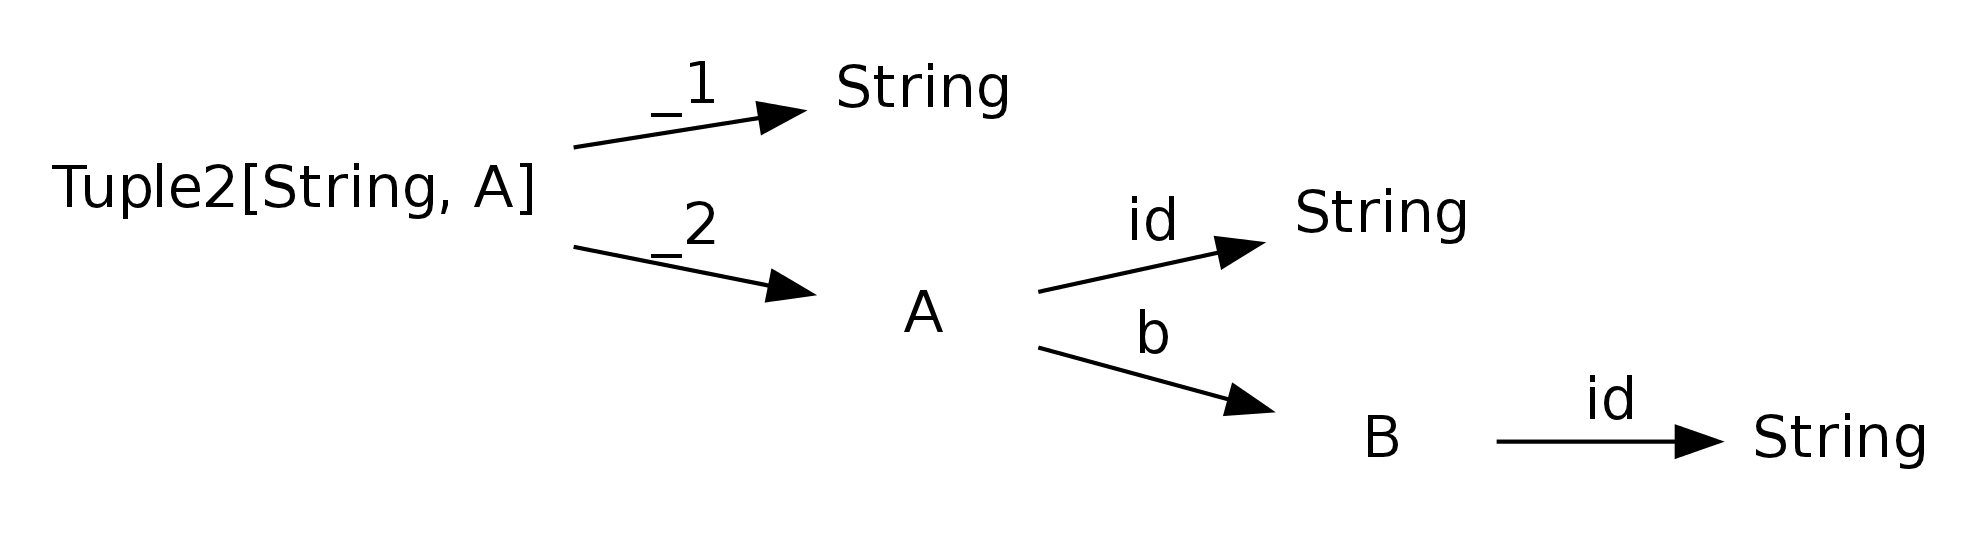
\includegraphics[clip=true, width=0.95\columnwidth]{dot/access.png}
\caption{Visualization of the tree of fields for class Tuple2[String, A]}
\label{fig:type_tree}
% \end{subfigure}
\end{figure}

% explaining the analysis
For each operation, we need to define how the access paths used by it are
translated into the access paths it uses. For this analysis we used following
primitives:
\begin{itemize}
\item \emph{Access paths for a type}: Given a type, this primitive creates
access paths for all the nested fields within it. This primitive can for example
be used to create the set of access paths needed for a \code{save} operation.
For the class \code{A}, it returns the access paths ${id, b, b.id}$.
\item \emph{Closure analysis}: This primitive analyzes a closure and returns a
set of all access paths relative to that closure's input type.
\item \emph{Rewrite access paths}: Several operations have semantics which
influence the type and therefore the access paths. For example, the \code{cache}
operation will always have the same input and output type and is known not to
change any fields, so all access paths from its successors must be propagated to
its predecessors. The \code{groupByKey} operation on the other hand always reads
all nested fields of the key, and has to rewrite all access paths of the value.
\item \emph{Narrow closure}: Given a closure, this primitive replaces the
closure's original output with a narrowed one based on the access paths of its
successors.
\end{itemize}

% \begin{table}[width=0.5\pagewidth, float=t]
% 
%     \begin{tabularx}{0.5\textwidth}{l|X|l}
%         Operation    & Propagate access paths 							     & Barrier \\ \hline
%         \code{filter}       & All access paths of successor + access paths of closure                                                      & ~       \\ 
%         \code{flatMap}      & Return closure analysis of narrowed closure                                             & ~       \\ 
%         \code{map}          & Return closure analysis of narrowed closure                                           & ~       \\ 
%         \code{join}         & Generates access paths all nested fields of the key, and propagates access paths to the values to the correct predecessor.    & x       \\ 
%         \code{groupByKey}   & Generates access paths all nested fields of the key, propagates the accesses to the value's iterable to the value itself  & x       \\ 
%         \code{reduce}       & All accesses from the closure are translated to accesses of the value's iterable and propagated        & ~       \\ 
%         \code{save}         & Generates all access paths for the input type           	                                             & ~       \\ 
%     \end{tabularx}
%     
%     \caption{Access path computation and propagation for selected operations.}
%     \label{table:field_reduction}
% \end{table}

\newcommand{\ar}{\Rightarrow}
\newcommand{\REWRITE}[3]{{rewrite(#1, \space #2 \ar #3)}}
\newcommand{\CA}[1]{analyze(#1)}
\newcommand{\CN}[1]{narrow(#1)}
\newcommand{\ALL}[1]{all(#1)}
\newcommand{\ENDTABLELINE}{}

\begin{table*} %[width=0.5\pagewidth, float=t]
    \begin{tabularx}{\textwidth}{l X c}
Operation & Access path computation and propagation & Barrier \\ \hline
\code{filter}	&	$P = S + \CA{f}$ & \\ \ENDTABLELINE
\code{map}		&	$P = \CA{\CN{f}}$  & \\ \ENDTABLELINE
\code{groupByKey}		&	$P = \ALL{I,\_1} + \REWRITE{S}{\_2.iterable.x}{\_2.x}$ & \checkmark \\ \ENDTABLELINE
\code{join}	&	$P_L = \ALL{I,\_1} + \REWRITE{S}{\_2.\_1.x}{\_2.x}$,  $P_R =
\ALL{I,\_1} + \REWRITE{S}{\_2.\_2.x}{\_2.x}$ & \checkmark \\	\ENDTABLELINE \code{reduce}	&	$P = \REWRITE{\CA{f}}{x}{\_2.iterable.x} +
\REWRITE{S}{\_2.x}{\_2.iterable.x}$ & \\ \ENDTABLELINE
% \code{reduce2}	&	$P = $ \newline $\REWRITE{CA(f)}{x}{\_2.iterable.x} + $ \newline $\REWRITE{S}{\_2.x}{\_2.iterable.x}$ & \\ \ENDTABLELINE 
\code{cache}	&	$P = S$ & \checkmark \\ \ENDTABLELINE
\code{save}	&	$P = \ALL{I}$ & \\ \ENDTABLELINE
\end{tabularx} 
    \caption{Access path computation and propagation for selected operations. 
    }
    \label{tbl:analysis}
\end{table*}


% make an example for map
To analyze a \code{map} operation, we need to combine the narrow closure and the
closure analysis primitive. The optimizations in LMS ensure that the output
symbol of a closure is always a constructor invocation. We apply the narrow
closure primitive to create a new closure, in which the new output reads from
the old output only the live fields. LMS recognizes when a field is read from a
constructor invocation in the same scope, and instead of generating an access
for a field, it returns that value directly. This happens for all the fields, therefore the old constructor
invocation will not be read anymore, and DCE will remove it. This means that the
field values, which only it was reading, will also not be read anymore, and they
too will be eliminated. When the closure has been cleaned of dead values, we can
analyze this new closure to get the access paths from it.

Table \ref{tbl:analysis} shows how relevant operations in \tool are
analyzed and how access paths are propagated. The first column is the operation
name, and the last column shows whether we treat this operation as a barrier. 
In the middle column we describe the rules for propagation of access paths. $P$
and $S$ are the access path sets of the predecessor and successor.
    $\CA{f}$ analyzes the given closure $f$, $\CN{f}$ narrows it.
    $\REWRITE{S}{x.y}{x.z}$ rewrites the access paths in $S$ with prefix $x.y$
    to have prefix $x.z$ instead.
    $I$ is the input element type of the operation, and $\ALL{I}$ can be used to
    generate the access paths.
